%%%%%%%%%%%%%%%%%%%%%%%%%%%%%%%%%%%%%%%%%
% NIWeek 2014 Poster by T. Reveyrand
% www.microwave.fr
% http://www.microwave.fr/LaTeX.html
% ---------------------------------------
% 
% Original template created by:
% Brian Amberg (baposter@brian-amberg.de)
%
% This template has been downloaded from:
% http://www.LaTeXTemplates.com
%
% License:
% CC BY-NC-SA 3.0 (http://creativecommons.org/licenses/by-nc-sa/3.0/)
%
%%%%%%%%%%%%%%%%%%%%%%%%%%%%%%%%%%%%%%%%%

%----------------------------------------------------------------------------------------
%	PACKAGES AND OTHER DOCUMENT CONFIGURATIONS
%----------------------------------------------------------------------------------------

\documentclass[a0paper,portrait]{baposter}

\usepackage[font=small,labelfont=bf]{caption} % Required for specifying captions to tables and figures
\usepackage{booktabs} % Horizontal rules in tables
\usepackage{relsize} % Used for making text smaller in some places

\usepackage{cmap}
\usepackage{mathtext}
\usepackage{icomma}

\usepackage[T1, T2A]{fontenc} % used to correctly output accented letters
\usepackage[russian, english]{babel}
\usepackage[utf8]{inputenc}

\usepackage{amsmath,amsfonts,amssymb,amsthm, mathtools} % Math packages
\usepackage{eqparbox}

\usepackage{textcomp}
\usepackage{multicol}
\usepackage{wrapfig} % Allows wrapping text around tables and figures

\graphicspath{{figures/}} % Directory in which figures are stored

 \definecolor{bordercol}{RGB}{40,40,140} % Border color of content boxes
 \definecolor{headercol1}{RGB}{0,51,153} % Background color for the header in the content boxes (left side)
 \definecolor{headercol2}{RGB}{0,51,153} % Background color for the header in the content boxes (right side)
 \definecolor{headerfontcol}{RGB}{226,226,226} % Text color for the header text in the content boxes
 \definecolor{boxcolor}{RGB}{226,226,226} % Background color for the content in the content boxes


\begin{document}

\background{ % Set the background to an image (background.pdf)
\begin{tikzpicture}[remember picture,overlay]
\draw (current page.north west)+(-2em,2em) node[anchor=north west]
{\includegraphics[height=1.1\textheight]{background}};
\end{tikzpicture}
}

\begin{poster}{
grid=false,
borderColor=bordercol, % Border color of content boxes
headerColorOne=headercol1, % Background color for the header in the content boxes (left side)
headerColorTwo=headercol2, % Background color for the header in the content boxes (right side)
headerFontColor=headerfontcol, % Text color for the header text in the content boxes
boxColorOne=boxcolor, % Background color for the content in the content boxes
headershape=roundedright, % Specify the rounded corner in the content box headers
headerfont=\Large\sf\bf, % Font modifiers for the text in the content box headers
textborder=rectangle,
background=user,
headerborder=open, % Change to closed for a line under the content box headers
boxshade=plain
}
{
\includegraphics[scale=0.45]{hse1.png}}
%
%----------------------------------------------------------------------------------------
%	TITLE AND AUTHOR NAME
%----------------------------------------------------------------------------------------
%
{ \bf  \huge {Производящие функции} }
%\Large \it A} % Poster title
{\vspace{0.3em} \smaller Кирилл Тамогашев, Иван Щекотови и Дмитрий Мячков \\для курса по Теории вероятности и статистике\\  % Author names
  
\smaller \it{Высшая Школа Экономики, Москва}} % Author email addresses
{
\includegraphics[scale=0.45]{hse1.png}} % University/lab logo

%----------------------------------------------------------------------------------------
%	ABSTRACT
%----------------------------------------------------------------------------------------
\headerbox{Введение}{name=abstract,column=0,row=0, span=3}{
\small{Приветствуем вас, дорогие любители математики! На этом плакате вы встретите определение производящей функции и узнаете о том, как производящие функции применяются в решении некоторых комбинаторных задач. В конце вас ждёт рекомендация отличного учебника по комибнаторике. Начнём же!}}


%----------------------------------------------------------------------------------------
%	Определение
%----------------------------------------------------------------------------------------
\headerbox{Определение}{name=definition,column=0,row=0,span=3,below=abstract}
{\small{Представим бесконечную последовательность чисел $\left\{a_i\right\}_{i=0}^\infty$. Можно записать ее
в качестве коэффициентов бесконечного полинома $f(t)$:
\[
	f(t) = \sum_{k=0}^{\infty} a_kt^k = a_0 + a_1t + a_2t^2 + \ldots
\]
$f(t)$ является производящей функцией. \\
\textbf{NB}: $f(t)$ является формальным степенным рядом, поэтому не обязательно, что представленный
ряд будет сходящимся. Нас интересуют коэффициенты, нежели чем переменные. \\
Самый простой пример производящей функции это геометрическая прогрессия:
\begin{align*}
	&a_0 = 1, a_n = qa_{n-1} \\
	1 + qt + &q^2t^2 + q^3t^3 + \ldots = \frac{1}{1 - qt}
.\end{align*}
}
}
%----------------------------------------------------------------------------------------
%	OTHER INSTRUMENTATION
%----------------------------------------------------------------------------------------
\headerbox{Числа Фибоначчи}{name=instruments,column=0,row=1,below=definition,span=1}
{
\small{
\textbf{Задача:} Сколькими различными способами можно разделить полоску, состящую из n ячеек, на полоски, состящие из одной или двух ячеек? 
Давайте разберёмся. 
Обозначим количество способов $f_n$ и докажем комбинаторно, что оно будет удовлетворять следующей реккуренте:
\[
	f_n = f_{n - 1} + f_{n - 2}
.\]
Отрежем от нашей полоски полоску из двух ячеек. 
Длина нашей новой полоски $n - 2$ ячейки.
Тогда число способов разделить оставшуюся часть полоски будет равно $f_{n - 2}$.
Теперь отрежем от исходной полоски полоску из одной ячейки.
По тем же соображение, количество способов поделить оставшуюся полоску будет равно $f_{n - 1}$.
И так далее, мы исчерпаем всевозможные способы разделить полоску на ячейки единичной длины и полоски из двух ячеек.

\bigskip
Заметим, что при $n = 1$: $f_1 = 1$, $n = 2$: $f_2 = 2$ и 
условимся, что для $n = 0$: $f_0 = 1$,
так как полоску нулевой длины можно разделить лишь одним способом – "никак".

Таким образом, мы доказали представленное выше реккурентное соотношение для известных чисел Фибоначчи.
\[
	F(s) = \sum_{n=0}^{\infty} f_ns^n = 1 + s + 2s^2 + 3s^3 + 5s^4 + \ldots
\]
Выведем замкнутую форму производящей функции:
\begin{align*}
	F(s) &= \sum_{n=0}^{\infty} f_ns^n = 1 + s + \sum_{n=2}^{\infty} f_ns^n = \\
	&= 1 + s + \sum_{n=2}^{\infty} (f_{n - 1} + f_{n - 2})s^n = \\ 
		 %&= 1 + s + s\left(\sum_{n=2}^{\infty} f_{n - 1}s^{n - 1}\right) +
	%s^2\left( \sum_{n=2}^{\infty} f_{n - 2}s^{n - 2} \right) = \\
		 %&= 
		 %1 + s + s\left(-1 + f_0 + \sum_{n=2}^{\infty} f_{n - 1}s^{n - 1}\right) +
		 %s^2\left( \sum_{n=2}^{\infty} f_{n - 2}s^{n - 2} \right) = \\
		 &=
		 1 + s + s\left(-1 + F(s)\right) + s^2F(s) = \\
		 &=
		 1 + sF(s) + s^2F(s) \\
	F(s) &= 1 + s + 2s^2 + 3s^3 + 5s^4 + \ldots = \\
	     &= 
	     \frac{1}{1 - s - s^2}.\text{ - производящая функция}
\end{align*}
}
}
%----------------------------------------------------------------------------------------
%	MIXER vs. SAMPLERS
%----------------------------------------------------------------------------------------
\headerbox{Пути}{name=paths,column=1,row=2,span=2,below=definition}{
\small{
\textbf{Задача:} Двигаясь только вправо или только вверх,
найти количество путей из $\left(0, 0\right) в \left(n, m\right)$.
Нетрудно убедиться, что таких путей $\binom{n + m}{m}$.
Найдем для них производящую функцию:
\begin{align*}
	A(x, y) =\sum_{n,m=0}^{\infty}\binom{n + m}{m}x^ny^m = 
\sum_{k = 0}^{\infty}\left( \sum_{m+n=k}^{\infty} \binom{n + m}{m}x^ny^m \right) =
\sum_{k=0}^{\infty} \left(x + y\right)^k = \dfrac{1}{1 - x - y} 
.\end{align*}
\begin{center}
    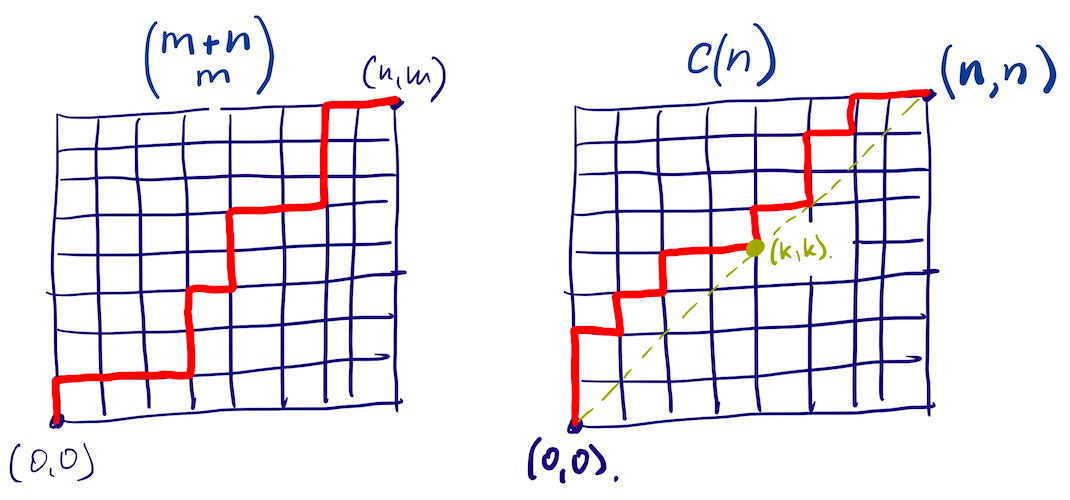
\includegraphics[scale=0.2]{path.jpg}
\end{center}

\subsection*{Числа Каталана}
Рассмотрим количество путей из $\left( 0, 0 \right) $ в $\left( n, n \right) $,
пролегающих выше прямой $y = x$. \\
Пусть $C(n)$ – искомое число путей. Тогда один из возможных способов дойти до
$\left(n, n\right) $ через точку $\left( k, k \right)$, где $k  \in \left[0, n\right)$ – это
все пути (их $C(k) $ штук) из $\left( 0, 0 \right) $ в $\left( k, k \right) $
умножить на все пути из $\left( k, k \right) $ в $\left( n, n \right) $, где их
$C(n - k - 1) $ штук. Тогда по всем имеющимся $k$ получаем реккурентное выражение для 
чисел Каталана:
\begin{align*}
	C(n) = \sum_{k=0}^{n - 1} C(k) \cdot  C(n - k - 1).
\end{align*}

Найдем для C(n) производящую функцию:
\begin{align*}
	K(q) &= \sum_{n=0}^{\infty} C(n)q^n = 1 + q + 2q^2 + 5q^3 + 14q^4 + \ldots = \ \left(?\right)\\
	K^2(q) &= \sum_{n=0}^{\infty}\left( \sum_{k=0}^{n - 1}C(k) \cdot C(n - k - 1) \right) q^n \\
	qK^2(q) & = \sum_{n=0}^{\infty}\left( \sum_{k=0}^{n - 1}C(k) \cdot C(n - k - 1) \right) q^{n + 1} =
	\sum_{n=1}^{\infty}\left( \sum_{k=0}^{n - 1}C(k) \cdot C(n - k - 1) \right) q^n \\
	qK^2(q) &= \sum_{n=1}^{\infty} C(n)q^n = K(q) - 1
.\end{align*}
Получив уравнение $qK^2(q) = K(q) - 1$, решим его для $K(q)$:
\[
	K(q) = \frac{1 - \sqrt{1 - 4q}}{2} \text{ – производящая функция для чисел Каталана.} 
\] 
}
}

%----------------------------------------------------------------------------------------
%	CONCLUSION
%----------------------------------------------------------------------------------------
\headerbox{Заключение}{name=conclusion,column=0,row=3,span=3,below=instruments,above=bottom}{\small{Мы хотели показать вам, как производящие функции связаны с некоторыми комбинаторными объектами и задачами. Однако, тема производящих функций очень обширна и выходит далеко за границы плаката. Всем заинтересовавшимся настоятельно рекомендуем познакомиться с книгой "Enumerative Combinatorics" под авторством гениального R.Stanley. Будет весело и страшно!}}

%----------------------------------------------------------------------------------------
%	REFERENCES
%----------------------------------------------------------------------------------------
%\headerbox{References}{name=references,column=1,below=conclusion,span=2}{

%}
%----------------------------------------------------------------------------------------
%	ACKNOWLEDGEMENTS
%----------------------------------------------------------------------------------------

\end{poster}
\end{document}